\section{Experiments}


\subsection{Deterministic Navier-Stokes}
\begin{figure}[h!t]
    \centering
    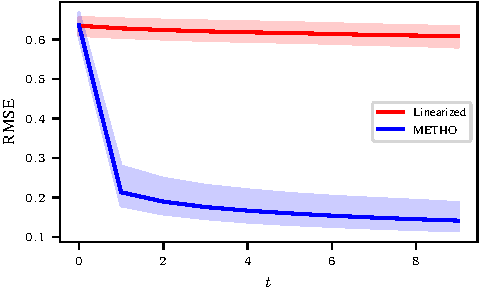
\includegraphics[scale=1]{linear_vs_metho_large.pdf}
    \centering
    \caption{Recovery of latent forcing in a Navier-stoke inversion problem. The plotted RMSE is unweighted \(\ell_2\) distance between MAP estimate \(\argmax \rho(\forcingst \gvn \mathcal{D}_t)\) and ground truth \(\forcingst\). Colored region denotes 90\% band over 80 realisations.}
    \label{fig:linear_vs_metho}
\end{figure}

We use a Navier-Stokes flow model on a 2-dimensional square domain with Neumann boundary conditions and inhomogenous forcing as depicted in Figure~\ref{fig:dynamicalsystem}.
The solver in this case has an heterogeneous acceleration term representing an external driving term \(\vrv{\forcing}\).
Both initial conditions and latent forcings are drawn from stationary Gaussian random fields with exponentially decaying spectrum.
Initial velocities are multiplied by an envelope term to ensure they satisfy Neumann boundary conditions.
For details see Appendix~\ref{app:pdes}.

In the deterministic setting the model is completely determined by initial conditions and latent parameters, and we may apply the method of linearisation to recover estimates of the unknown \(\vrv{\forcing}\).

We apply \meth{} with an ensemble size of 400, \(\sigma^2=10^{-4}\) and the linearised method with \(\sigma^2=0.1\), and compare each method in terms of the \(\ell_2\) error between the MAP estimate and ground truth, on a spatial grid of size \(128\times 128\).
Results are plotted in Figure~\ref{fig:linear_vs_metho}.
Although both are able to iteratively improve the error in this metric, the linearised method is drastically less data-efficient in that the solution improves less with each time step, as we would expect for a large \(\sigma^2\).
On the other hand, setting \(\sigma^2\) to a smaller number results in unstable inference, with solutions not improving or even diverging.

Timings reflect inference on NVIDIA P100 GPUs, implemented in pytorch.
The 90\% range of simulation time (i.e. running the prediction model) for the linearised method was $18$-$24$ seconds and for \meth{} was $2.6$--$3$ seconds.
We note, however, that the linearised method is possibly unfairly penalised by the inefficient implementation of multivariate Jacobians in the version of pytorch used.
The 90\% range for the inference time for the linearised method in was $0.13$-$0.26$ seconds and for the \meth{} was $0.027$--$0.064$ seconds.

\subsection{Stochastic Navier-Stokes}

In the stochastic case the Navier-Stoke solver is perturbed by adding a spatially homogeneous, centred, white Gaussian noise \(\vrv{\nu}_t\) term to the each element of the velocity vector before applying the forward prediction operator of the Navier-Stoke solver.
In this stochastic setting we cannot apply the linearised method.
Moreover, in this problem the solution grid is of dimension \(512 \times 512\), which causes the covariance matrices to be too large for inference on common hardware.

In this challenging setting we test the influence of the ensemble size upon the quality of \meth{} inference.
For each ensemble size we conduct 80 replicates over 5 observation updates.
Results are plotted in Figure~\ref{fig:n_ens}.

Because the likelihood (and therefore the posterior) is not ever explicitly formed in this black-box forward model and is in any case intractable, it is difficult to evaluate the exact posterior density assigned to the ground truth parameter $\forcingst^\ast$.
That is, we cannot evaluate $p(\forcingst^\ast \gvn \mathcal{D}_T)$.
However, all else being equal, assigning a high value to the approximate posterior density $\rho(\forcingst^\ast \gvn \mathcal{D}_T)$ evaluated at $\forcingst^\ast$ is indicative of a higher quality model.
In Figure~\ref{fig:n_ens} we plot $\rho(\forcingst^\ast \gvn \mathcal{D}_t)$ as a function of ensemble size $N$.
We see a gradual improvement then plateau in all metrics as the size of the ensemble grows, although selecting the precise trade-off is problem-dependent.

% \begin{figure*}[h!t]
%      \centering
%     \begin{subfigure}{0.48\textwidth}
%          \centering
%          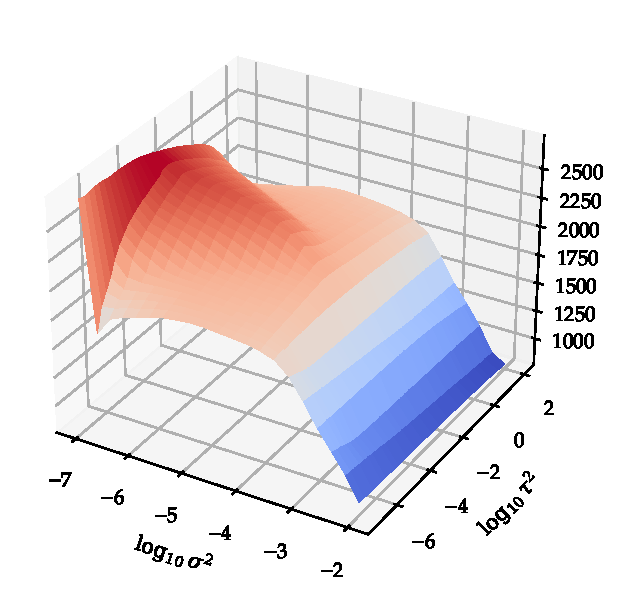
\includegraphics[scale=0.75]{meth_hyp_ens_5_Prob_surf.pdf}
%          \caption{Median estimated posterior probability}
%          \label{fig:tau2sig2_prob}
%      \end{subfigure}
%      \begin{subfigure}{0.48\textwidth}
%          \centering
%         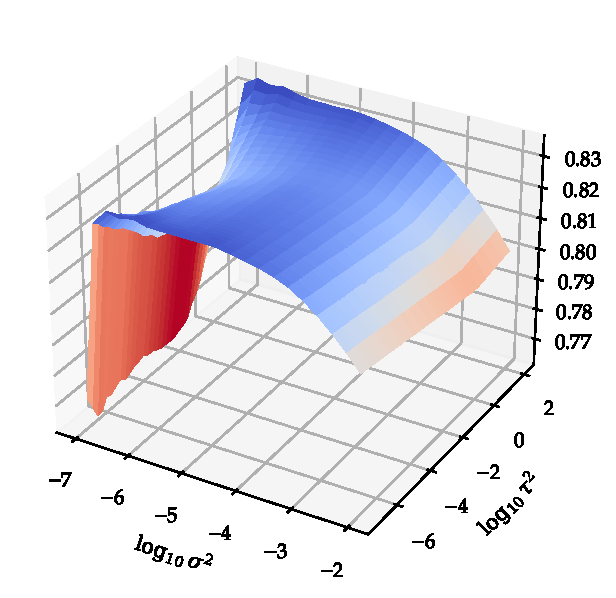
\includegraphics[scale=0.75]{meth_hyp_ens_5_RMSE_surf.pdf}
%          \caption{Median estimated RMSE of the posterior mean from the ground truth}
%          \label{fig:tau2sig2_rmse}
%      \end{subfigure}
%      % \hfill
%     \centering
%     \caption{Effect of hyperparameters on estimates of true forcing $\forcing$ under \meth{}, 80 replicates of 5 observations.}
%     \label{fig:tau2sig2}
% \end{figure*}

\begin{figure}[h!t]
    \centering
     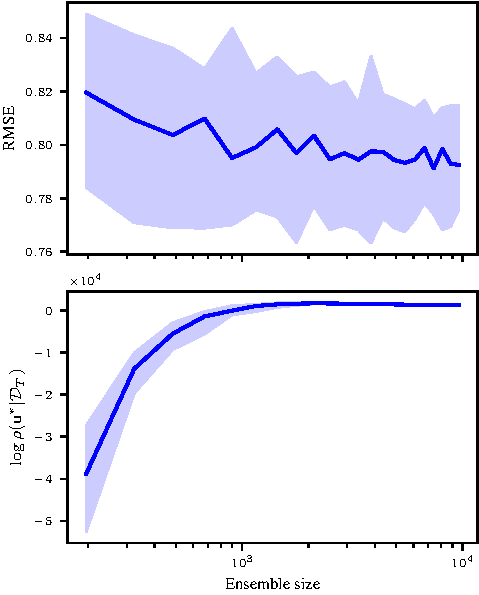
\includegraphics[scale=1]{meth_ex_ens_5.pdf}
    \centering
    \caption{Effect of ensemble size on model RMSE and estimated likelihood. 80 replicates of 5 observations, i.e. \(T=4\). Shaded region shows empirical 90\% range, dark line shows median.}
    \label{fig:n_ens}
\end{figure}
